\cotefile{12}
\scanpage{99}
\deleted{\uline{Introduction}} \mspage{1.}

\uline{Filtration} \uline{et poids} \uline{\deleted{\unsure{pour}} des espaces de cohomologie} \uline{des variétés algébriques}

0. Introduction

1. Notion du \uline{poids} \inserted{et notion du \uline{niveau}} pour un \deleted{\unsure{pro}}module \inserted{pro} Galoisien sur un corps. \deleted{\unsure{exemples}}

2. Étude d'un schéma privé d'un diviseur à croisements normaux.

3. Poids \inserted{et niveau} de $H_{\deleted{\unsure{!|*|c}}}^{i}(X)$ ($X$ lisse)

4. Poids \inserted{et niveau} de $H^{i}_{!}(X)$ ($X$ séparé). \deleted{\unsure{Cas|Cor}}

\deleted{\unsure{5.}} 5. Poids et niveau des $H^i(X)$ ($X$ quelconque)

6. Cas $X$ propre : \inserted{le plus grand} quotient de $H^i(X)$ de poids $i$, et résolution des singularités. \deleted{Application}.

7. Cas $X$ propre et lisse : filtration de $X$ par les niveaux.

\deleted{\unsure{8.|7.}} Nombres de Betti virtuels de Serre.

8. Contre\unsure{-}exemples divers.

9. Cas des coefficients tordus \ldots

\noindent\rule{\linewidth}{0.4pt}

[\unsure{1|*}] SGA 4

[ ] P. Deligne / Hodge

[ ] Tate / conjectures

[ ] \unsure{Kleimann|Kleinmann|Kleiman} \quad conj. \unsure{standart|standard}

[ ] Weil \quad conj

[ ] Deligne. Grothendieck \quad \uline{SGA 7}
% archive sheet number: 98
\scanpage{101}
\[
\left\{\begin{aligned}
 X&=\mathbb{P}^{2}-T'\\
 Y&=T-T'\\
 U&=\mathbb{P}^{2}-T
\end{aligned}\right.
\]

\figure{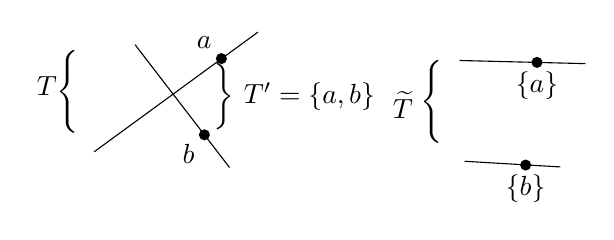
\begin{tikzpicture}[x=.8cm,y=.8cm]
\node at (-.75,1.05) {$T$};
\node at (-.42,.95) {$\Biggl\{$};
\draw (0,0)--(2.6,1.9);
\draw (.65,1.7)--(2.15,-.25);
\fill (2.02,1.48) circle (2pt) node[above left] {$a$};
\fill (1.75,.27) circle (2pt) node[below left] {$b$};
\node at (2.06,.87) {$\biggr\}$};
\node[right] at (2.22,.87) {$T'=\{a,b\}$};
\node at (4.9,.75) {$\widetilde T$};
\node at (5.35,.8) {$\Biggl\{$};
\draw (5.8,1.45)--(7.8,1.40);
\draw (5.88,-.15)--(7.4,-.24);
\fill (7.03,1.42) circle (2pt) node[below] {$\{a\}$};
\fill (6.85,-.21) circle (2pt) node[below] {$\{b\}$};
\end{tikzpicture}}

\diagram{\begin{tikzcd}[ampersand replacement=\&,column sep=small]
H^1(\widetilde Y)\deleted{\unsure{\leftarrow|=}}\arrow[dr] \& \& \\
H^3_Y(X)\arrow[r] \& H^{3}_{\deleted{\unsure{!|Y}}}(X)\arrow[r,dash] \& H^3(U)
\end{tikzcd}}

\diagram{\begin{tikzcd}[ampersand replacement=\&,column sep=small]
H^1_!(Y) \& H^1_!(X)\arrow[l]\arrow[dl] \& H^1_!(U)\arrow[l] \& H^0(\\
H^1_!(\widetilde Y) \& \& {\substack{\Vert\\0\ \text{car }T\ \text{connexe}}}
\end{tikzcd}}

\diagram{\begin{tikzcd}[ampersand replacement=\&,column sep=small,row sep=small]
H^0(\widetilde T')\arrow[r] \& H^0_{\unsure{!|1|{}}}(\widetilde T)\arrow[r] \& H^1_!(\widetilde Y)\arrow[r] \& H^1(\widetilde T')\\
H^0(\mathbb P^2)\arrow[r]\arrow[u] \& H^0_{\unsure{!|{}}}(T')\arrow[r]\arrow[u] \& H^1_!(X)\arrow[r]\arrow[u] \& {\underset{\substack{\Vert\\\unsure{0|1|{}}}}{H^1(\mathbb P^2)}}\arrow[u]\\
H^0(P^2)\arrow[r] \& H^0(T)\arrow[r]\arrow[u] \& H^1_!(U)\arrow[r]\arrow[u] \& {\underset{\substack{\Vert\\\unsure{0|1|{}}}}{H^1(P^2)}}
\end{tikzcd}}

\margin{$\left\{\begin{aligned}&T\ \text{\uline{connexe}}\\ &T'\ \text{disconnexe, \deleted{et}}\end{aligned}\right.$ contenu \unsure{ds|dans} \unsure{lieu|lieux}. \deleted{\unsure{lieu}} de lissité, et tte comp. de $T'$ contient au plus un point de $T'$.}

\diagram{\begin{tikzcd}[ampersand replacement=\&,column sep=tiny,row sep=large]
\& \& H^0(T')/\operatorname{Im}H^0(\mathbb P^2)\arrow[dl,"{\text{\unsure{inj|isog|isom} ?}}"] \& {\underset{\substack{\Vert\\0}}{H^0(T)/\operatorname{Im} H^0(\mathbb P^2)}}\arrow[l]\\
H^1_!(\widetilde Y)\ \unsure{\supset|\rightarrow} \& {H^0(\widetilde T/\operatorname{Im}H^0(\widetilde T')\,{}_{\ =0}} \& \&
\end{tikzcd}}

\[
\deleted{\unsure{H^1_!|H^1_4}}
\]
\noindent\rule{\linewidth}{0.4pt}
% archive sheet number: 100
\scanpage{104}
\margin{\unsure{!}}

\diagram{$\begin{array}{c@{\quad}ccc}
 &\multicolumn{2}{c}{\overbrace{\hphantom{\text{poids 0}\qquad\text{poids 1}}}^{\text{\deleted{\unsure{pour}} \quad cas propre, ou du }H^1_!}}&\\
 H^1&\text{poids }0&\text{poids }1&\text{poids }2\\
 &\text{niveau }0&\text{niveau }1&\text{niveau }0\\
 &&\multicolumn{2}{c}{\underbrace{\hphantom{\text{niveau 1}\qquad\text{niveau 0}}}_{\text{cas lisse}}}
\end{array}$}
\margin{morceaux purs sont semi-simples}

\diagram{$\begin{array}{c@{\quad}c|ccccc}
 \multicolumn{2}{c}{}&\multicolumn{3}{c}{\overbrace{\hphantom{0\qquad1\qquad2}}^{\text{cas propre}}}&&\\
 H^2_{\deleted{\unsure{!}}}&\uline{\text{poids}}&0&1&2&3&4\\
 &\text{niveau}&0&1&2&1&0\\
 \multicolumn{2}{c}{}&&&\multicolumn{3}{c}{\underbrace{\hphantom{2\qquad1\qquad0}}_{\text{cas lisse}}}
\end{array}$}

morceaux purs de poids $\ne 2$ sont semi-simples.

$\Vert$ Le morceau pur de poids $2$ est une extension par un motif de Tate $Q(-1)^{r}$.

$H^2_!$ \quad il semble qu'il puisse y avoir mélange de poids dans le mauvais \unsure{rdre|ordre|sens}, à cause d'une extension d'un motif \unsure{effectif|affectif} de poids $0$ par un autre de poids $1$ ; en plus de cela, il apparaît une extension, peut-être non triviale, d'un motif effectif de poids $0$ \inserted{resp. $1$} par un autre.
% archive sheet number: 103
\scanpage{105}
% The heading is enclosed in a hand-drawn frame.
\uline{Poids de la cohomologie \inserted{$l$-adique} d'une variété singulière ou/et non propre \inserted{(sur corps $k$ parfait)}.}

\textcircled{A} \uline{Coefficients constants}

\textcircled{1} Soit d'abord $X$ lisse et quasi-projective, donc par résolution forte (que nous admettons) on aura
\[
 X=X'-Y \qquad Y=\bigcup_i Y_i
\]
$X'$ lisse et projective, $Y_i$ diviseurs lisses \inserted{irréd.} à croisements normaux mutuels. \deleted{\unsure{Soit}} On a donc
\[
\begin{aligned}
\inserted{H^{i-1}(X')\to H^{i-1}_{\unsure{!|{}}}(Y)}&\\[-3pt]
\deleted{\unsure{R^if_!}}&\to H^i_!(X)\to H^i(X')\to H^i(Y)\to H^{i+1}_!(X)\to\ldots
\end{aligned}
\]

% Small diagram in the left margin.
\diagram{\begin{tikzcd}[ampersand replacement=\&,row sep=small,column sep=small]
X\arrow[r,phantom,"\subset"]\arrow[d,"f"'] \& X'\arrow[dl,"f'"]\\
\operatorname{Sp}\unsure{_{\mathrm e}|{}|\mathrm{ec}}\,k \&
\end{tikzcd}}

\deleted{\unsure{donc}} donc les poids dans $H^i_!(X)$ (qui se déterminent via val. absolues de val. propres de Frob, par réduction au cas d'un corps de type fini \ldots) est contenu dans ceux de $H^i(X')$ [réduits à $i$ par Weil] et ceux de $H^{i-1}(Y)$.

Or on
\[
 H^*(Y)\Longleftarrow E_2^{pq}
 =H^p\bigl(\unsure{i_0\ldots i_r|i_0\ldots i_p}\longmapsto H^q(Y_{i_0}\cap\ldots\cap Y_{i_{\unsure{r|p}}})\bigr)
 \left\{\begin{aligned}
 &\text{de poids }q\\
 &\text{de niveau }\le q\\
 &[\text{intervient si }\\[-2pt]
 &i=p+q)\le n-1]\\
 &\text{de niveau }\le\unsure{2n-i-q}\\
 &\inserted{\unsure{-q|{-}p}}\\
 &[\unsure{\text{et}|\text{si}}\, i=p+q\ge n]
 \end{aligned}\right.
\]
\margin{$(2n-i-1)-q$}
\margin{(on peut se borner ici aux cochaînes \uline{alternées}}

\deleted{Donc} Or ici $Y_{i_0}\cap\ldots\cap Y_{i_p}$ est projectif et lisse (de dimension $n-p-1$ si $X$ \deleted{\unsure{connexe}} purement de dim $n$).

Donc le poids du terme $E^{pq}_2$ est $q$, et on trouve que le poids de $H^j(Y)$ est $\le j$. Donc :

\deleted{\uline{\unsure{Lemme 1|Lemme}}} \inserted{\uline{Proposition 1}} $H^i_!(X)$ est de poids \inserted{entre $0$ et} $\le i$. La partie de poids $i$ (resp. de poids $\le i-1$) est le quotient image de $H^i_!(X)\to H^i(X')$ [resp l'image de $H^{i-1}(Y)\to H^i_!(X))$. De plus, si $i\ge n=\dim X$, alors le \uline{niveau} de $H^i_!(X)$ est $\le 2n-i$, et les \unsure{deuxièmes|derniers|deux} morceaux précédents sont de niveau $\le 2n-i-1$ ; de plus, il n'y a de poids qu'entre $2(i-n)$ [car il faut écrire $q\le 2(n-p-1)$ !] et $i$, i-e sur un intervalle d'amplitude $2n-i$ !\ldots

\margin{\uline{NB} Tous les morceaux de la filtration sont \textquotedblleft effectifs\textquotedblright}
\margin{En tous cas, niveau $\le\operatorname{Inf}(i,n)$}

Pour ce complément, notons que le niveau de $E^{pq}_2$ est $\le$ celui de $H^q(\underbrace{Y_{i_0}\cap\ldots\cap Y_{i_p}}_{\dim n-p-1})$, donc est
\[
\begin{aligned}
 {}\le{}&\deleted{\unsure{\operatorname{Inf}(q,}}\,2(\deleted{\unsure{\dim}}n-p-1)-q\,\unsure{\bigr)|\}|{}}\\
 ={}&\deleted{\unsure{\operatorname{Inf}(q,}}(2n-i-2)-p
 \inserted{\deleted{\unsure{2q}}=2(n-1)-i-p}
 \quad(\inserted{\text{si }}i=p+q)\ \text{donc }\le 2(n-1)-i
\end{aligned}
\]
% archive sheet number: 104
\scanpage{106}
Donc \deleted{\unsure{en posant|remplaçant}} pour $p+q=i-1$, on trouve un poids $\le 2(n-1)-i+1=2n-i-1$.

\uline{Remarque} \quad La filtration de $H^*(Y)$ déduite de la suite spectrale \unsure{$\infty$|SS|ci} n'est autre que la filtration par les poids. La filtration image de $H^i_!$ est donc aussi la filtration par les poids croissants (de $0$ à $i$, le dernier cran \unsure{comme|connu} noyau) donc est également indépendante de la \unsure{compactification} $X'$ choisie. Écrivons les termes de la filtration, en utilisant le fait que $H^{i-1}(X')$ est purement de poids $i-1$, et \deleted{$E_2^{i-1,0}$} que la suite spectrale $\infty$ dégénère pour des raisons de poids :

\diagram{$\begin{array}{c|c|c|c|c|c|c}
\hline
 &E_2^{i-1,0},&E_2^{i-2,1},&\ldots&E_2^{1,i-2},&
 E_2^{0,i-1}/\operatorname{Im}H^{i-1}(X'),&
 \operatorname{Ker}(H^i(X')\to E_2^{0,i})\\ \hline
 \text{poids}&0&1&&i-2&i-1&i\\ \hline\hline
 \deleted{\text{\unsure{niveau}}}&&&&&&
\end{array}$}

\deleted{\unsure{Car si on|Cas $i\ge n$}} Si $i\le n$, les \textquotedblleft{}niveaux sont \inserted{\unsure{seult|seulm.}} $\le$ poids, il n'y a pas lieu à priori d'attendre plus. L'on trouve d'autre part, pour $i\ge n$, un tableau

\diagram{$\begin{array}{c|c|c|c|c|c|c}
 &\overset{\text{\unsure{degré filtrant|de gr. filtré} }\ge n}{0\quad\ldots\quad0}
 &E_2^{\substack{\deleted{\unsure{2n-i,\,i-1}}\\2n-i-1,2(i-n)}}
 &E_2^{2n-i-2,2(i-n)+1}&\ldots
 &E_2^{0,i-1}/\operatorname{Im} H^{i-1}(X')&
 \operatorname{Ker}(H^i(X')\to E_2^{0,\unsure{i}})\\ \hline
 \text{poids}&\smash{\raisebox{-.7ex}{$\times$}}&2(i-n)&2(i-n)+1&\ldots&i-1&i\\ \hline
 \text{niveau}&&0&1&\ldots&2n-i-1&2n-i
\end{array}$}

\uline{Corollaire 1} \quad (Par dualité) $H^i(X)$ est de poids compris entre $i$ et $2n$\deleted{\unsure{$-i$}}. Le morceau \deleted{\unsure{pur}} de poids $i$ est exactement l'image de $H^i(X')$. Si $i\deleted{\unsure{<}}\ge n$, les niveaux des morceaux de poids $i,i+1,\ldots,2n$ sont resp. $\le 2n-i,2n-i-1,\ldots,0$. Si $i\le n$, il n'y a de morceaux \deleted{\unsure{de}} que des poids \deleted{$i,i+1,\ldots,2n-2(n-i)=2n$\unsure{ $2i$, \ldots, dont}} \inserted{$i,i+1,\ldots,2i$} qui sont de niveaux resp. $\le i,i-1,\ldots,0$.

% slanted
\margin{Tous les morceaux de la filtration sont \textquotedblleft\uline{effectifs}\textquotedblright}
% slanted
\margin{En tous cas niveau $\le\operatorname{Inf}(i,n)$}
\margin{\uline{NB} les niveaux ici \uline{décroissent}}
% archive sheet number: 105
\scanpage{107}
\textcircled{2} \uline{Cas \deleted{\unsure{du}} lisse non quasi-projectif.}

Si $X$ est séparé, utilisant une compactification de Nagata, et résolution des singularités \inserted{comme dessus}, on a les \deleted{\unsure{ms}} résultats que ci-dessus, en notant que la résolution des singularités permet de déduire les \unsure{conj.|Conj.} de Weil pour des var. propres et lisses du cas projectif et lisse.

Si $X$ non séparé, $H^i_!(X)$ n'est plus défini. Par contre $H^i(X)$ est défini. On a, avec un recouvt affine
\[
 H^*(X)\Longleftarrow E^{pq}_2=H^p(\sigma\longleftarrow H^q(U_\sigma))
\]
Ici $E^{pq}_2$ est effectif de poids $\ge q$, mais \deleted{\unsure{on déduit peut-être ainsi|non dégénéré}} on peut en conclure que l'effectivité de $H^i(X)$, et le fait que ces poids sont compris entre $0$ et $2n$ si $i\ge n$, et entre $0$ et $2i$ si $i\le n$ ; en tous cas, ces poids sont $\le 2i$, \deleted{\unsure{enfin, le ni}}. Enfin, on trouve que le niveau est $\le i$ \deleted{\unsure{et sera donc resp. et $\le 2n-i$} (il suffit de regarder pour $i>n$)}

\margin{\uline{Question} le niveau est-il $\le 2n-i$ ? \deleted{\unsure{pour $X$ non séparé}}}
\margin{\unsure{ici|où|si} $n=\dim X$}

\textcircled{3} \uline{Cas non lisse} : $H^i_!(X)$, ($X$ séparé). Je dis qu'il est encore vrai qu'il est \uline{effectif} et de poids $\le i$, de niveau $\le\operatorname{Inf}(i,2n-i)$ ! Soit $U$ un ouvert lisse dense, $Y$ son complémentaire.

Donc
\[
 \to H^i_!(U,\unsure{\mathbb Q_\ell|{}})\to H^i_!(X)\to H^i_!(Y)\to
\]
et $H^i_!(U)$\deleted{\unsure{est}} est effectif de poids $\le i$ \inserted{de niveau $\le i$}, et $H^i_!(Y)$ aussi par hypothèse de récurrence sur la dimension, donc $H^i_!(X)$ est effectif de poids $\le i$, de niveau $\le i$. De \unsure{m} $H^i_!(U)$ est de niveau $\le 2n-i$, et $H^i_!(Y)$ de niveau $\le 2(n-1)-i\le 2n-i$, on gagne.

\textcircled{4} \uline{Cas non lisse} : $H^i(X)$ \deleted{\unsure{($X$ séparé)} \unsure{?}}. Je dis qu'il est effectif, à poids $\le\underline{\underline{2i}}$, à niveau \deleted{\unsure{$\le\operatorname{Inf}(i,n)$ où $n=\dim X$}} \inserted{$\le i$ et $\le n$}. \inserted{Par la suite spectrale de Leray, on est ramené au cas où $X$ affine.} Récurrence sur $i$, trivial si $i\le 0$. On utilise résolution $X'\to X$, et suite spectrale de descente
\[
 H^*(X)\Longleftarrow E_2^{pq}=H^p(s\longmapsto H^q((X'_{/X})^s))
\]
\margin{poids $\le 2\operatorname{Inf}(i,n)$}
\margin{niveau $\le\operatorname{Inf}(i,n)$}
\deleted{\unsure{si}} Par hyp. de récurrence, \deleted{\unsure{pour}} \inserted{si $q<i$}, $E_2^{pq}$ est effectif
% archive sheet number: 106
\scanpage{108}
de \deleted{niveau} poids $\le 2q$, de niveau $\le q$. Donc il en est ainsi de $E^{rs}_2$ si $p+q=i$, $p\ne 0$, \inserted{et ce terme est de \deleted{\unsure{poids, de}} poids $\le 2(i-1)<2i$, de niveau $\le i-1<i$} Reste à examiner le terme $E^{0,i}_2\subset H^i(X')$ ; comme $X'$ est lisse, il est donc effectif, de poids $\le 2i$, de niveau $\le i$. On gagne\unsure{!}, si on note que si $i>n$, on a $H^i(X)=0$ ($X$ affine !).

\deleted{Si $X$ \unsure{propre ;|provenait ;|fortiori} $H^i(X)$ est de niveau $\le n=\dim X$. Il suffit \unsure{de l'éprouver pour les} $E_2^{pq}$. \unsure{Il suffit d'utiliser un recouvt}}

\textcircled{B} \uline{Coefficients constants tordus sur $X$ lisse} \inserted{séparé}, $F$ \inserted{effectif} de poids et \inserted{niveau $j$.}

\textcircled{1} On suppose que les coefficients envisagés proviennent d'un motif lisse sur $X$, et \inserted{\unsure{par dévissage (possible loc ?)|par dévissages (possible loc ?)}} on va regarder le cas où ce dernier est un facteur direct d'un $R^jf_*(\mathbb Q_{\ell Y})$, avec $f:\deleted{\unsure{X}}Y\to X$ morphisme projectif et lisse. \inserted{On peut si on veut supposer $f$ de dim relative $j$.} On est donc ramené au cas où $F=R^jf_*(Q_{\ell Y})$. \inserted{On} Considérons la suite spectrale
\[
 H^*(Y)\deleted{\unsure{\Leftarrow}}\Longleftarrow \inserted{E^{pq}_2=}H^p(X,R^q f_*(Y))
\]

\uuline{D'après Deligne,} cette suite spectrale dégénère. Donc $H^i(X,R^jf_*(Q_{\ell Y}))$ \inserted{et par suite $H^i(X,F)$} apparait comme un \uline{morceau} de $H^{i+j}(Y)$. On trouve que l'on a un \deleted{module} \uline{effectif}, de poids \deleted{\unsure{\#}} compris entre \deleted{\unsure{$0$}} \deleted{$2(n+j)$ et $2(i+j)$} \uline{$i+j$} et $2(n+j)=\underline{2n+2j}$ (où $n=\dim X$) ; les niveaux sont resp. $\le(2n-i+j),\ldots,0$.
\margin{peut-on remplacer $2n+2j$ par $2n+j$ ?}

Si $i\le n$, il n'y a de poids \unsure{qui ont|qu'en} les dimensions $i+j,i+j+1,\ldots,\bigl(2(i+j)\bigr)$, de \deleted{poids} \inserted{niveaux} respectifs \deleted{\unsure{$2i,\ldots,i+j$|$\le 0,\ldots,i+j$}.} \inserted{$i+j,i+j-1,\ldots,0$}
\margin{peut-on remplacer $2i+2j$ par $2i+j$ ? \deleted{\unsure{Il doit faire ça pour|Idiot \illegible{3}}} !}

Résultats duels pour $H^i_!(F)$, il est effectif à poids $\le i+j$, et \deleted{à niveaux} si $i\ge n$, il est à niveaux croiss. de de $0$ à \deleted{$2n-i+j$} $2(n+j)-(i+j)=2n-i+j$. \inserted{pour des poids croissants de}
\margin{les poids sont-ils $\ge j$ \deleted{\unsure{resp.}}}

Si $X$ est \uline{propre}, on trouve que $H^i(X,F)$ est pur de poids $i+j$ (et semi-simple ici\ldots, !
% archive sheet number: 107
\scanpage{109}
\textcircled{2} Cas où on dispose seulement d'une représentation de $F$ sous forme sympathique \uline{localement} sur $X$ pour la top. (Zar). Dans ce cas, \deleted{on ne peut plus utiliser \unsure{comme} l'hyp. $X$ séparé, on doit en tous cas localiser sur $X$ au sens (ét), et utiliser la suite spectrale de Leray d'un recouvrement. On trouve \unsure{au moins} l'effectivité, poids entre $0$ et $2n+2j$}
on a intérêt à travailler \uline{d'abord} avec la cohomologie à support propre sur $X$, qui permet de découper $X$ en morceaux, et d'obtenir le $=$ résultat que dessus. On déduit l'analogue en cohomologie à supports quelconques par dualité.

\deleted{Si $F$ est sympathique,}
\uline{Remarque} [ En fait, on voit par ce raisonnement que, en ce qui concerne la coh. à support propre, les résultats sont obtenus en supposant seulement que $F$ soit \textquotedblleft joli par morceaux\textquotedblright{} sur $X$ ; \inserted{\unsure{la lissité|se lissité} de $X$ \unsure{pas nécessaire|par récurrence|par ailleurs}} ]. Le fait $F$ constant tordu \inserted{sur $X$ lisse} est alors utilisé \deleted{\unsure{dans le cas li}} pour pouvoir procéder par dualité.

\textcircled{C} \uline{Cas de coefficients effectifs de (poids} $j$, \uline{niveau} $j$) \uline{quelc.}, $X$ quelconque.

1) Cas de la cohomologie $H^i_!$ : déjà traité dans la remarque précé\deleted{\unsure{dente}}dente : résultat le $=$ que dans \textcircled{B}.1).

2) Cas de la cohomologie $H^i(X,F)$. Je dis qu'il est \uline{effectif}, de poids \deleted{entre $0$ et $2i$}, \inserted{$\le\operatorname{Inf}(2i,2n)=2\operatorname{Inf}(i,n)$}, de niveau $\le\operatorname{Inf}(i,n)$, où $n=\dim X$. \deleted{On procède par} \ldots
\margin{?}
% archive sheet number: 108
\scanpage{111}
Faisceaux $l$-adiques admissibles et motifs virtuels.

\deleted{1. Soit $S$ un schéma, $F$ un \unsure{$Q_l$|$\mathbb Q_\ell$}}

1. On se fixe un nb premier $l$. Les schémas envisagés sont premiers à $l$. (\uline{Le cas le plus intéressant est celui des schémas} loc. de \uline{type fini sur $\mathbb Z$}.) Les faisceaux envisagés sont les $Q_l$-faisceaux \inserted{constructibles}. On note $Q_l(1)$ le faisceau de Tate $T_l(G_m)\otimes_{\mathbb Z_l}Q_l$, et le twist par sa puissance tensorielle $n$ième est noté $F\longmapsto F(n)$.

% slanted
\margin{se borner pour commencer à ce cas !}
% slanted
\margin{On travaille dans la catégorie des \textquotedblleft faisceaux $l$-adiques de nature arithmétique\ldots}
% slanted
\margin{définition concrète : dire qu'on se ramène à une situation de t.f. sur $\operatorname{Sp}\mathbb Z$}

2.1 Un faisceau $F$ sur $S$ est dit \uline{spécial} \inserted{\uline{de poids} $i$} s'il est isomorphe à un \deleted{facteur direct} \inserted{quotient \deleted{\unsure{constant}} tordu} d'un \inserted{sous} faisceau \inserted{constant tordu d'un faisceau} de la forme $R^i f_*(Q_{lX})$, où $f:X\to S$ est projectif et lisse \inserted{de dim relative $\unsure{i|j}$ \unsure{plutôt ?}}. \unsure{(|[}On notera que si $i<0$, cela implique $F=0$ ; si $i=0$, cela \deleted{\unsure{équivaut} \unsure{implique}} équivaut à : $F$ localement constant.$^{(+)}$

% slanted
\margin{\deleted{\unsure{Attention}, la réciproque n'est pas vraie ; même pour un groupe fini seulement, il faut une repr. sur $Q$, et \unsure{pas que} \illegible{2} \uline{\unsure{définissable sur $Q$}} !}}

\uline{Lemme} 2.\unsure{1|2}. \quad a) Stabilité de \textquotedblleft spécial de poids $i$\textquotedblright{} par \inserted{sous-\unsure{facteurs|quotients} et quotients cst tordus, et} sommes directes.

b) Si $F,F'$ sont spéciaux de poids respectifs $i,j$, alors $F\otimes F'$ est spécial de $i+j$.

c) Stabilité par images inverses.

d) Si $F$ spécial de poids $i$, $\check F(-i)$ l'est aussi

e) $Q_l(-i)$ est spécial de poids $\deleted{\unsure{-|a}}\unsure{2i|i}$ pour $i\ge0$

a) se prouve en introduisant un $\coprod_{1\le i\le n}X_i$.

b) se prouve en considérant un $X_1\times_S X_2$, et utilisant Künneth

c) Par th. de changement de base.

\margin{d) utiliser Lefschetz}

d) \uline{Par th. de Lefschetz} en cohomologie $l$-adique.

e) On \deleted{peut} a $Q_l(-i)=R^{2i}f_*(Q_{l\mathbb P^i_S})$.

\margin{\uline{Cor} 2\unsure{?|3} Si $F$ spécial de poids $i$, et $n\ge i$, alors $\check F(-n)$ est spécial de poids $2n-i$}

3.1 Un faisceau $F$ sur $S$ est dit \uline{effectivement} \uline{admissible} si \inserted{pour tout ouvert affine $U$ de $S$} on peut en trouver une \deleted{filtration de $F$\unsure{$|S$|$|U$} dont les quotients} \inserted{filtration \deleted{de \unsure{$F|U$}} de $F|U$ dont les quotients} successifs sont de la forme $i_!(G)$, où $i:Y\to X$ est une \deleted{\unsure{et de la forme} $i_!(\phantom G)$ \unsure{d'une partie de $U$ en partie}} imm. de présentation finie et où $G$ sur \unsure{$S_Y$|$Y$} est \deleted{\unsure{solution} localement isomorphes \unsure{constructibles} \unsure{pour les $F|S$ sont|pour les $F|S_\alpha$ sont}} admissible.

\margin{il faut se permettre une extension finie surj. loc. libres radicielles de $Y$, pour rendre $G$ spécial}

\deleted{On dit} Si $P$ est une partie de $\mathbb Z$, on dit que $F$ est à poids $\subset P$ si \deleted{les \unsure{$F|S_i$|$F|S_\alpha$} sont} \inserted{on peut prendre les $G$} admissibles de poids $\in P$. (\uline{Donc} \deleted{eff. admissible} alors $F$ est de poids $\in P'$, pour tt $P'\supset P$). Si \deleted{\unsure{$P\subset E$ et $P=\varnothing$, cela implique}} $P$ ne contient pas d'entier $\ge0$, cela implique $F=0$

% slanted
\margin{Attention, il n'est pas tautologique que si $F$ est eff. adm à poids $\in P$ et à poids $\in P'$, il soit : \deleted{\unsure{$P\cap P'$}} poids $\in P\cap P'$, \unsure{même si} $P\cap P'=\varnothing$}
% archive sheet number: 110
\scanpage{112}
\deleted{a) Si $F$ spécial de \unsure{pds|poids}}

\uline{Proposition} 3.3 \quad a) Stabilité de \textquotedblleft eff. adm. de poids $\subset P$\textquotedblright{} par sous-faisceau constructible, quotient constructible, \inserted{sommes finies,} extensions.

b) Si $F,F'$ sont eff. adm à poids $\subset P,P'$, alors $F\otimes F'$ est admissible à poids $\subset P+P'=\{i+i'\mid i\in P,i'\in P'\}$.

c) Stabilité par chgt de base

d) Si $F$ est \deleted{spécial} eff$^{\mathrm t}$ admissible \uline{constant} \uline{tordu} à poids $\subset P$, \deleted{\unsure{et}} si $i\in P\Rightarrow i\le n$, alors $\check F(\unsure{-n|n})$ est à \inserted{eff$^{\mathrm t}$} admissible (constant tordu) à poids $\subset 2n-P=\{n-i\mid i\in P\}$.
\margin{d) modulo Lefschetz}

\uline{Dém} \quad a) b) c) sont immédiats, on utilise les assertions correspondantes de 2.1. Notons d'ailleurs :

% Left of 3.2; the arrowhead is beside the top line of the sheet.
\figure{\begin{tikzpicture}[x=.42cm,y=.33cm]
\draw[->] (1,0) .. controls (1.5,2.8) and (-2,6.4) .. (-1,8.3) .. controls (-.7,9.0) and (.2,9.6) .. (.7,9.8);
\draw (1.8,.5) .. controls (.8,.4) and (.9,-.7) .. (.9,-1.1) -- (.9,-3.0) .. controls (.9,-3.6) and (1.2,-3.6) .. (1.8,-3.45);
\end{tikzpicture}}
3.2. \inserted{Supposons $S$ qu. cpt qu. sép.} Pour que $F$ soit eff$^{\mathrm t}$ adm. à poids $\subset P$, il f et s. que l'on puisse trouver une partition de $S$ en \deleted{\unsure{fermés}} sous-schémas $S_i\overset{\alpha_i}{\lhook\joinrel\longrightarrow} S$, $\alpha_i$ imm. de prés. finie, avec \deleted{\unsure{des}} $F|S_i=F_i$ admettant une filtration dont les quotients successifs sont spéciaux de poids $\in P$.

Comme, pour $F$ constant tordu, la formation de $\check F$ commute au changement de base, \inserted{3.\unsure{2|?}} d) résulte de 2.2.

4.1 Un faisceau $F$ est dit eff$^{\mathrm t}$ admissible \deleted{\unsure{poids}} de niveaux $\le\unsure{\nu|v}$ si \deleted{il est effectivement admissible, et} dans 3.1, on peut prendre $G$ \deleted{\unsure{de poids $j\in$}} de la forme $G'(-k)$, $k\ge0$ où $G'$ est spécial de poids \deleted{\unsure{$j$}} $\le\nu$, \deleted{\unsure{on|---}} On dit que $F$ est eff$^{\mathrm t}$ admissible \textquotedblleft de poids $\subset P$, et de niveau $\le\nu$\textquotedblright{} si on peut choisir dans 3.1. $G'$ \deleted{\unsure{à la}} spécial de poids $j\le\nu$, avec \deleted{\unsure{poids $G$}} $j+2k\in P$. \uline{Attention}, à priori cela est plus fort que la \uline{conjonction} de \textquotedblleft de poids $\subset P$\textquotedblright{} et \textquotedblleft de niveau $\le\nu$\textquotedblright. \deleted{\unsure{Pour cette notion conjointe, on a un énoncé :} \unsure{4.2 a) b) c) d)|4.2 a) b) c)}} \inserted{On notera que si \deleted{\unsure{$P\le\nu$}}, $\nu$ est} un entier tel que $P\le\nu$ (i.e $j\in P\Rightarrow j\le\nu$), alors \textquotedblleft eff$^{\mathrm t}$ adm. de poids $\in P$\textquotedblright{} $\to$ \textquotedblleft id et à niveau $\le\nu$\textquotedblright

% slanted
\margin{bloquer après 3.2, avec \unsure{énoncé analogue} : 3.2, pour faire sortir 3.3 en $=$ temps que 4.2.}
% archive sheet number: 111
\scanpage{113}
\uline{Proposition} 4.2 \deleted{\unsure{a)}} a) Stabilité de \textquotedblleft eff$^{\mathrm t}$. adm. de poids $\subset P$ et niveau $\leq\unsure{\nu|v}$\textquotedblright\ par sous-faisceau constr., quotients constructibles, sommes finies, extensions.

b) $F_i$ \textquotedblleft eff. adm de poids $\subset P_i$, niveau $\leq\nu_i$\textquotedblright\ pour $i=1,2$ implique $F_1\otimes F_2$ \textquotedblleft eff$^{\mathrm t}$. adm. de poids $\subset P_1+P_2$, niveau $\leq\nu_1+\nu_2$\textquotedblright.

c) Stabilité par chang$^{\mathrm{mt}}$ de base.

d) Si $F$ \inserted{eff$^{\mathrm t}$} admissible \uline{constant tordu} \textquotedblleft à poids $\deleted{\unsure{\leq q|k}}\inserted{\nu+2k}$ et niveau $\leq\nu$\textquotedblright, \deleted{et si}\inserted{(où $k\geq0$, $\nu\geq0$)}, alors pour tout $n\geq\nu+k$\inserted{ (soit $n=\nu+k+h$, $h\geq0$)}, $\check F(-n)$ est \textquotedblleft eff$^{\mathrm t}$. admissible constant tordu, à poids $2n-\nu-2k=\nu+2h$, niveau $\leq\nu$\textquotedblright.

\uline{\unsure{Remarks|Remarq|Remarque}}: introduire plutôt: \textquotedblleft à morceaux de poids $i_\alpha$, niveau $\nu_\alpha$\textquotedblright, $\alpha\in\ldots$\textquotedblright.

\margin{\uline{Utiliser Lefschetz} \uline{ou Deligne}}
% slanted
\uline{Théorème} 5.1. Soit $f:X\longrightarrow S$ morphisme séparé de \deleted{\unsure{t.f.|type}}\inserted{prés finie}, et $F$ \deleted{eff$^{\mathrm t}$ admissible \unsure{de niveau de poids} \unsure{facteur}}\inserted{\uline{strictement spécial} de poids $j$} sur $X$ (i.e. déf. 1 s'applique, avec $F$ \uline{facteur direct} d'un $R^jg_*(Q_{lY})$, où $g:Y\longrightarrow X$ \deleted{\unsure{de}}\inserted{proj. lisse}). \deleted{\unsure{(i.e. déf. 2.1, est de poids $\subset P$, niveau|(i.e. déf. 2.1, avec} \illegible{2}} Alors $R^if_!(F)$ est \uline{eff$^{\mathrm t}$ admissible} \deleted{\unsure{constructible}}\inserted{à poids $\leq$\deleted{\unsure{q}}$i+j$ \deleted{\unsure{et}} et niveaux $\leq\operatorname{Inf}(i+j,2n-i+j)$} \deleted{poids $\unsure{\leq i+j}$ \unsure{si $f$ est lisse et $X$ est} \unsure{de dim. relative $n$}, de niveau \unsure{$i+j$}. Si $n=\operatorname{Sup}\dim X_s$, et si $i\geq n$, alors les poids}.

\margin{$+$ résolution des singularités forte sur les schémas parfaits, aux corps résiduels de $S$.}
% slanted
\margin{$+$ $\frac12$ simplicité \unsure{arithmétiques|arithmétique} ?}
% slanted
Si $n=\operatorname{Sup}_{s\in S}\dim X_s$, \deleted{\unsure{ses}} et si $i\geq n$, les poids \deleted{\unsure{et}} et niveaux \deleted{\unsure{sont}} possibles sont
\diagram{\[
\begin{array}{c|c|c|c|c|}
\text{poids}&2(i-n)&2(i-n)+1&\ldots&(i+j)\\ \hline
\text{niveaux}&\leq0&\leq1&\ldots&\leq2n-i+j
\end{array}
\]}

\uline{Démonstration} On \deleted{\unsure{en|(a)}} peut supposer $F=R^jg_*(Q_{lY})$, $g:Y\longrightarrow X$ proj. lisse. \deleted{\illegible{2}} Utilisant le th. de chang$^{\mathrm{mt}}$ de base propre, \deleted{\illegible{2}} et dévissage via suite exacte de cohomologie à support propre, on est ramené au cas où \deleted{$\exists\, S'\longrightarrow S$} $S$ est affine, \unsure{nell$^{\mathrm e}$|nlle|noeth.}, intègre, $\exists\, S'\longrightarrow S$ morphisme fini plat radiciel, \inserted{$X$ affine,} tel que $X'=X\times_S S'$ est \uline{lisse} sur $S'$, et se \textquotedblleft compactifie\textquotedblright\ en un $\widehat X_{S'}$ \deleted{tel que $X'$} projectif et lisse, tel que $\widehat X_{S'}-X_{S'}$ soit un diviseur à croisements normaux relatifs, à \unsure{compos$^{\mathrm{tes}}$|composantes} irréductibles \uline{lisses} sur $S'$; \inserted{enfin $F$ \deleted{\unsure{sur}} \illegible{1}} \inserted{étant \uline{spécial} de poids $j$.} Quitte à changer de notation, on peut supposer $S=S'$, \deleted{et} d'où $X\subset X'=\hat X$. On trouvera alors, \inserted{si $F=Q_{lX}$,} comme dans les notes préliminaires (partie A, 1)). [\uline{NB} On n'utilise pas la dégénérescence de la suite spectrale qui y intervient.]
\margin{à expliciter ce point en utilisant successiv$^{\mathrm{mt}}$ \unsure{corollaire de} 3.3. a) et 4.2 a)}
% slanted
% archive sheet number: 112
\scanpage{114}
\deleted{B) Cas général. On se réduit au}

Si $F$ est quelconque, on écrit que $F$ est un sous-\deleted{quotient d'un \inserted{\unsure{ct tordu|ct. tordu}} quotient \inserted{\unsure{ct tordu}} d'un $R^df_*(Q_{lY})$}, où $f:Y\longrightarrow X$ morphisme projectif. [Utilisant Lefschetz \deleted{et 2.1 de \unsure{$f$, $f'$} \unsure{is. à une section de $f$}, faible, on peut supposer que les fibres de $f$ \unsure{sont de dim $j$}]} \deleted{\unsure{fort|fortement}} si $j<d=\dim$ relative de $Y/X$, et remplaçant $Y$ par $Y\times_X\mathbb P_X^{j-d}$ si $j>d$, on peut supposer $j=d$]
\margin{\deleted{\unsure{par Lefschetz fort.|Lefschetz fort.}}}
% slanted
\margin{voir si cette réduction est vraiment utile\ldots}
% slanted

La suite spectrale
\[
 R^\alpha_!(fg)(Q_l)\Longleftarrow E_2^{pq}=R^p_!f(R^q_!g(Q_{lX}))
\]
dégénère \uline{par Deligne}, donc
\[
\begin{aligned}
 R^i_!f(F)=E^{ij}_2\quad &\text{est }\simeq\text{ quotient \inserted{c$^{\mathrm t}$. tordu} d'un ss-faisceau ct}\\
 &\text{tordu d'un }R^{i+\unsure{j|g}}_!g(Q_{lY}).
\end{aligned}
\]
\margin{\uuline{utiliser Lefschetz fort}}
% slanted
\margin{[N.B. Voir si Deligne ne peut se remplacer ici par \uline{factorisation d'}\uline{Artin} sur $X\longrightarrow S$, pour revenir au cas de $n=1$\ldots]}
% slanted
La conclusion en résulte, en utilisant le cas précédent pour $Y\longrightarrow S$, de dim relative $\leq n+j$ \ldots

\uline{Corollaire} 5.2. Si la partie \uuline{\textquotedblleft semi-simplicité\textquotedblright} des conjectures de Tate est vérifiée, la conclusion de 5.1. est vraie dès que l'on suppose seulement que $F$ est eff$^{\mathrm t}$. admissible de poids $j$. Par suite, si on suppose $F$ eff$^{\mathrm t}$. admissible de poids $\leq\deleted{\unsure{q}}\inserted{j}$, on a un énoncé correspondant, \deleted{\unsure{De ce}} $R^if_!(F)$ est \inserted{eff. admissible,} \deleted{de} poids $\leq\deleted{\unsure{\operatorname{Inf}(i+j,2n-i+j)}}\unsure{i+j}$, \inserted{niveau $\leq\operatorname{Inf}(i+j,2n-i+j)$.} Si $i\geq n$, on trouve des poids entre $2(i-n)$ et $i+j$, correspondant aux niveaux $0,1,\ldots,\unsure{2-i+j|2n-i+j}$.
\margin{semi-simplicité utilisée!}
% slanted; the note is circled.

(On se ramène en effet \inserted{par dévissages et déf.} au cas où $F$ est \uline{spécial} de poids $j$, et par th. de chgt. de base propre au cas où $S$ de type fini sur Spec $\mathbb Z$, et \unsure{ainsi de suite}\deleted{\unsure{au cas où}})

\uline{Cor.} 5.3 (sous conj. type Tate) \deleted{\unsure{on a aussi}} Si $F$ est eff. admissible, Alors $R^i_!f(F)$ est eff$^{\mathrm t}$. admissible.
\margin{Alors par semi-simplicité $F$ est $=$ str$^{\mathrm t}$ spécial}
% slanted
% archive sheet number: 113
